\documentclass[aspectratio=169]{beamer}
\usetheme[numbering=fraction]{metropolis}

% ── Ruban titre ───────────────────────────────────────────────
\makeatletter
\setlength{\metropolis@frametitle@padding}{1ex}
\makeatother

% ── Suppression des slides de transition de section ──────────
\metroset{sectionpage=none}

\usepackage[french]{babel}
\usepackage[T1]{fontenc}
\usepackage[utf8]{inputenc}
\usepackage{lmodern}
\usepackage{csquotes}
\usepackage{xcolor}
\usepackage{graphicx}
\usepackage{booktabs}
\usepackage{caption}
\usepackage{tikz}
\usetikzlibrary{arrows.meta,positioning,calc,decorations.pathmorphing}
\usepackage{varwidth}
\usepackage{colortbl}
\usepackage{array}
\usepackage{amsmath}
\usepackage{appendixnumberbeamer}
\graphicspath{{../../../results/sechilienne/figures/}{./}}

% ================================================================
% COULEURS
% ================================================================
\definecolor{myblue}{HTML}{1F4E79}
\definecolor{myblue2}{HTML}{2E6BA8}
\definecolor{myorange}{HTML}{E07B39}
\definecolor{mygreen}{HTML}{2E7D32}
\definecolor{myred}{HTML}{C0392B}
\definecolor{myteal}{HTML}{006064}
\definecolor{mylgray}{HTML}{F4F6F9}
\definecolor{mymgray}{HTML}{D0D8E4}
\definecolor{mydgray}{HTML}{4A5568}
% bandes radar (mêmes couleurs que les figures)
\definecolor{Lband}{HTML}{2E7D32}
\definecolor{Cband}{HTML}{7B4FA8}
\definecolor{cut}{HTML}{C0392B}
\definecolor{ctrl}{HTML}{1F77B4}

% ================================================================
% COULEURS BEAMER
% ================================================================
\setbeamercolor{frametitle}{bg=myblue, fg=white}
\setbeamercolor{progress bar}{fg=myblue, bg=gray!20}
\setbeamercolor{block title}{bg=myblue, fg=white}
\setbeamercolor{block body}{bg=mylgray}
\setbeamercolor{block title alerted}{bg=myorange, fg=white}
\setbeamercolor{block body alerted}{bg=mylgray}
\setbeamercolor{block title example}{bg=mygreen, fg=white}
\setbeamercolor{block body example}{bg=mylgray}
\setbeamercolor{alerted text}{fg=myorange}
\setbeamercolor{bibliography entry author}{fg=myblue}
\setbeamercolor{bibliography entry title}{fg=myblue}

\captionsetup{labelfont=bf, font=small}

\newcommand{\Lb}[1]{\textcolor{Lband}{\textbf{#1}}}
\newcommand{\Cb}[1]{\textcolor{Cband}{\textbf{#1}}}

% ================================================================
% COMMANDE SOUS-TITRE DE SLIDE
% ================================================================
\newcommand{\slidesubtitle}[1]{%
	\textcolor{myblue}{\small\textbf{#1}}%
	\par\vspace{3pt}%
}
% chiffre clé : couleur, valeur, légende
\newcommand{\keynum}[3]{%
	\begin{minipage}[t]{0.31\linewidth}\centering
		\textcolor{#1}{\Large\textbf{#2}}\\[1pt]
		\scriptsize #3
	\end{minipage}}

% ================================================================
% BIBLIOGRAPHIE
% ================================================================
\usepackage[backend=biber, style=authoryear,
maxcitenames=2, mincitenames=1,
isbn=false, eprint=false, doi=false, url=false]{biblatex}
\addbibresource{../../latex/references.bib}

\AtBeginDocument{%
	\renewcommand*{\mkbibnamefamily}[1]{\textnormal{#1}}%
	\renewcommand*{\mkbibnamegiven}[1]{\textnormal{#1}}%
	\renewcommand*{\mkbibnameprefix}[1]{\textnormal{#1}}%
	\renewcommand*{\mkbibnamesuffix}[1]{\textnormal{#1}}%
}
\DeclareCiteCommand{\parencite}
{\usebibmacro{prenote}}
{\textcolor{black}{(}\textcolor{myred}{\usebibmacro{cite}}\textcolor{black}{)}}
{\multicitedelim}
{\usebibmacro{postnote}}

% ================================================================
% PIED DE PAGE
% ================================================================
\setbeamercolor{footline}{bg=white, fg=black}
\setbeamerfont{footline}{size=\scriptsize}
\setbeamertemplate{footline}{%
	\hbox{%
		\begin{beamercolorbox}[wd=\paperwidth, ht=1.5ex,
			dp=0.6ex, leftskip=0.4cm,
			rightskip=0.4cm]{footline}
			\color{black}\rule{\paperwidth}{0.3pt}\par
			\vspace{-0.25em}
			\hfill \insertframenumber/\inserttotalframenumber
		\end{beamercolorbox}%
	}%
}

% ================================================================
% PAGE DE TITRE PERSONNALISEE
% ================================================================
\setbeamertemplate{title page}{%
	\begin{tikzpicture}[overlay, remember picture]
		\node[anchor=north west, xshift=0.5cm, yshift=-0.45cm]
		at (current page.north west)
		{
\includegraphics[height=0.9cm]{../../presentation/logos/logo_icube.png}};
		\node[anchor=north east, xshift=-0.5cm, yshift=-0.35cm]
		at (current page.north east)
		{
\includegraphics[height=1.3cm]{../../presentation/logos/logo_sertit.png}};
	\end{tikzpicture}%
	\vspace*{1.1cm}
	\vfill
	\begin{center}
		\footnotesize\textcolor{mydgray}{%
			Dossier de candidature -- Stage SERTIT / ICube (Université de Strasbourg)}

		\vspace{0.3em}
		\scriptsize\textcolor{mydgray}{%
			\og Exploration des bandes L et P (NISAR, BIOMASS) pour la détection de la déforestation
			et des glissements de terrain \fg}

		\vspace{0.9em}

		\begin{varwidth}{0.92\linewidth}
			\centering
			{\usebeamerfont{title}\usebeamercolor[fg]{title}%
				\inserttitle\par}
		\end{varwidth}

		\vspace{0.6cm}

		{\usebeamerfont{author}\usebeamercolor[fg]{author}%
			\insertauthor\par}

		\vspace{0.4cm}

		{\usebeamerfont{date}\usebeamercolor[fg]{date}%
			\insertdate\par}
	\end{center}
	\vfill
}

\title{\Large
	Bande L (NISAR) contre bande C (Sentinel-1)\\
	sur un glissement boisé : Séchilienne\\[4pt]
	{\normalsize la phase radar traverse-t-elle la forêt ? (version réduite)}
}
\author{%
	Candidat : \textbf{Mamadou G. Diallo}
}
\date{Novembre 2026}

% ================================================================
\begin{document}

\begin{frame}
	\titlepage
\end{frame}

% ================================================================
\section{Question et site}
% ================================================================

\begin{frame}{\phantom{x}}
	\frametitle{Question et site}
	\vspace{-6pt}\scriptsize
	\begin{columns}[T]
		\column{0.40\textwidth}
		\begin{block}{Question}
			\scriptsize
			Sur un versant \textbf{boisé} et instable, la bande \Lb{L} garde-t-elle une phase
			interférométrique exploitable là où la bande \Cb{C} la perd ?
		\end{block}
		\begin{block}{Séchilienne (Isère)}
			\scriptsize
			\begin{itemize}
				\setlength{\itemsep}{0pt}
				\item Flanc SE du Mont Sec, 450--1\,140~m, très surveillé
				\item Zone frontale (éboulis nus) : très active dans les années 2010, ralentie depuis
				\item Reste du versant : de l'ordre du cm/an, sous la forêt
			\end{itemize}
		\end{block}
		\column{0.58\textwidth}
		\centering
		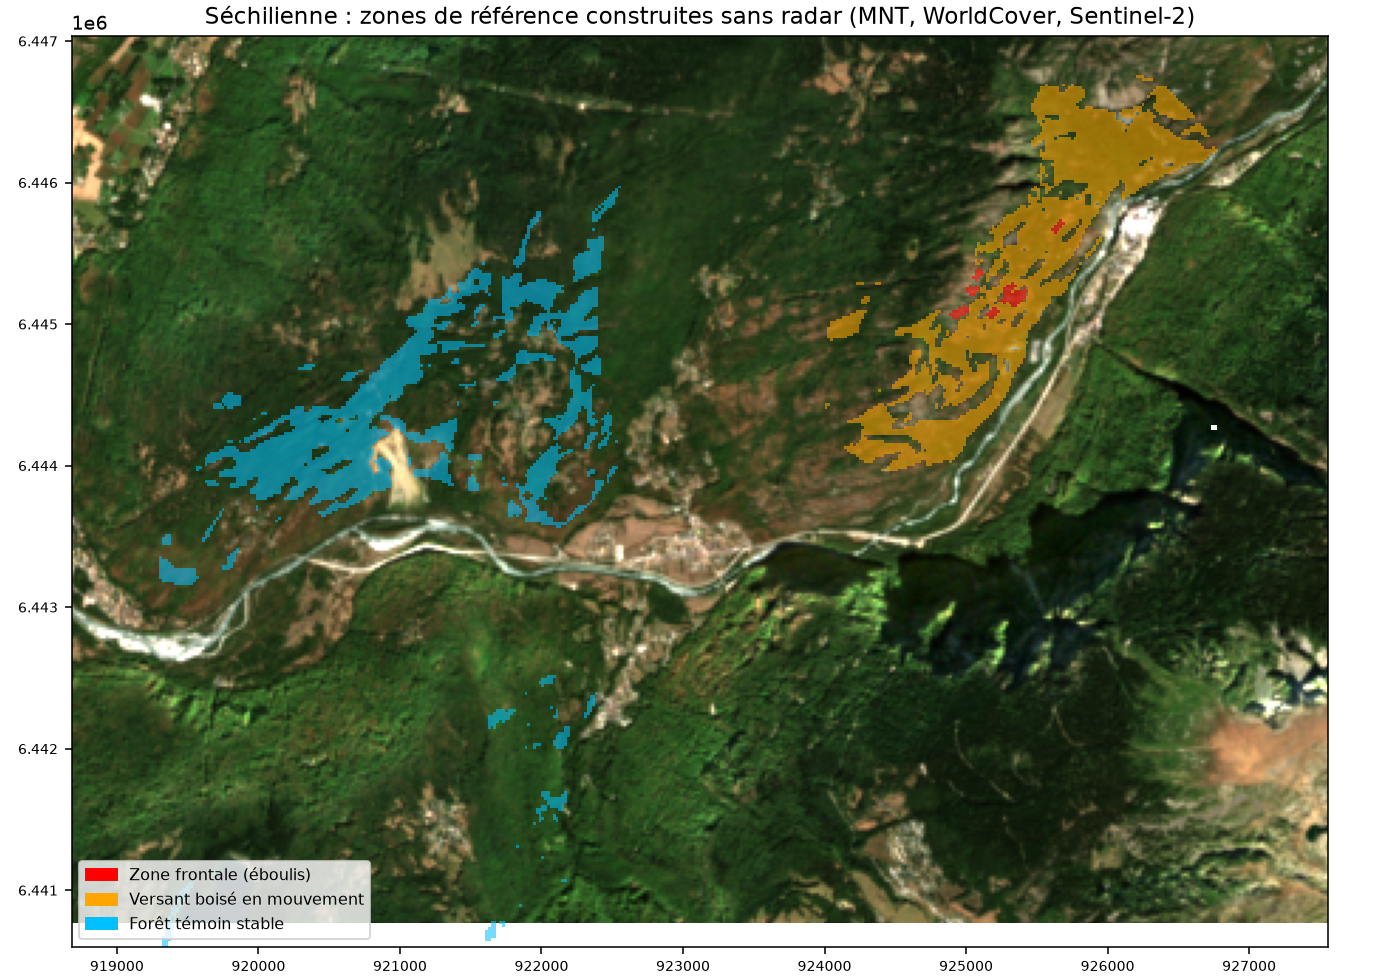
\includegraphics[width=\linewidth, height=0.60\textheight, keepaspectratio]{g1b_zones.png}
		\begin{block}{Zones construites sans radar}
			\scriptsize
			Sources : MNT, WorldCover \parencite{zanaga2022worldcover}, Sentinel-2, littérature\\
			\textcolor{cut}{frontale} 4,6~ha -- versant 168~ha (pente 40°) -- \textcolor{ctrl}{témoin} 160~ha (36°, à plus de 2,5~km)
		\end{block}
	\end{columns}
\end{frame}

\begin{frame}{\phantom{x}}
	\frametitle{Données et méthode}
	\vspace{-6pt}\scriptsize
	\begin{columns}[T]
		\column{0.50\textwidth}
		\begin{block}{17 paires appariées, 26/06 -- 24/10/2026}
			\scriptsize
			\begin{itemize}
				\setlength{\itemsep}{0pt}
				\item \Lb{NISAR} \parencite{kellogg2020nisar} GUNW (\textbf{ISCE3}) \parencite{isce3} : A173 (9) et D138 (8)
				\item \Cb{Sentinel-1} \parencite{torres2012sentinel1} IW SLC, VV : A161 et D139, mêmes paires (écart $\leq$ 2~j)
				\item Interférogrammes \Cb{C} sous SNAP \parencite{snap} (graphe réutilisable, sans ESD)
				\item 1 cycle = 11,9~cm (\Lb{L}) contre 2,8~cm (\Cb{C}) en distance
			\end{itemize}
		\end{block}
		\column{0.48\textwidth}
		\begin{block}{Indicateurs par zone}
			\scriptsize
			\begin{itemize}
				\setlength{\itemsep}{0pt}
				\item Cohérence médiane
				\item \textbf{Consistance de phase} $|\langle e^{j\varphi}\rangle|$ après référencement
				sur le témoin : 1 = phase commune, 0 = bruit
				\item \Lb{L} : variation de distance cumulée, rampe et troposphère stratifiée retirées
			\end{itemize}
		\end{block}
		\begin{alertblock}{Contrôle de la chaîne C}
			\scriptsize
			Cohérence \Cb{C} de 0,97--0,99 sur le bâti : le traitement est correct.
		\end{alertblock}
	\end{columns}
\end{frame}

% ================================================================
\section{Résultats}
% ================================================================

\begin{frame}{\phantom{x}}
	\frametitle{Résultats (1/3) : cartes, géométrie montante}
	\vspace{-6pt}
	\centering
	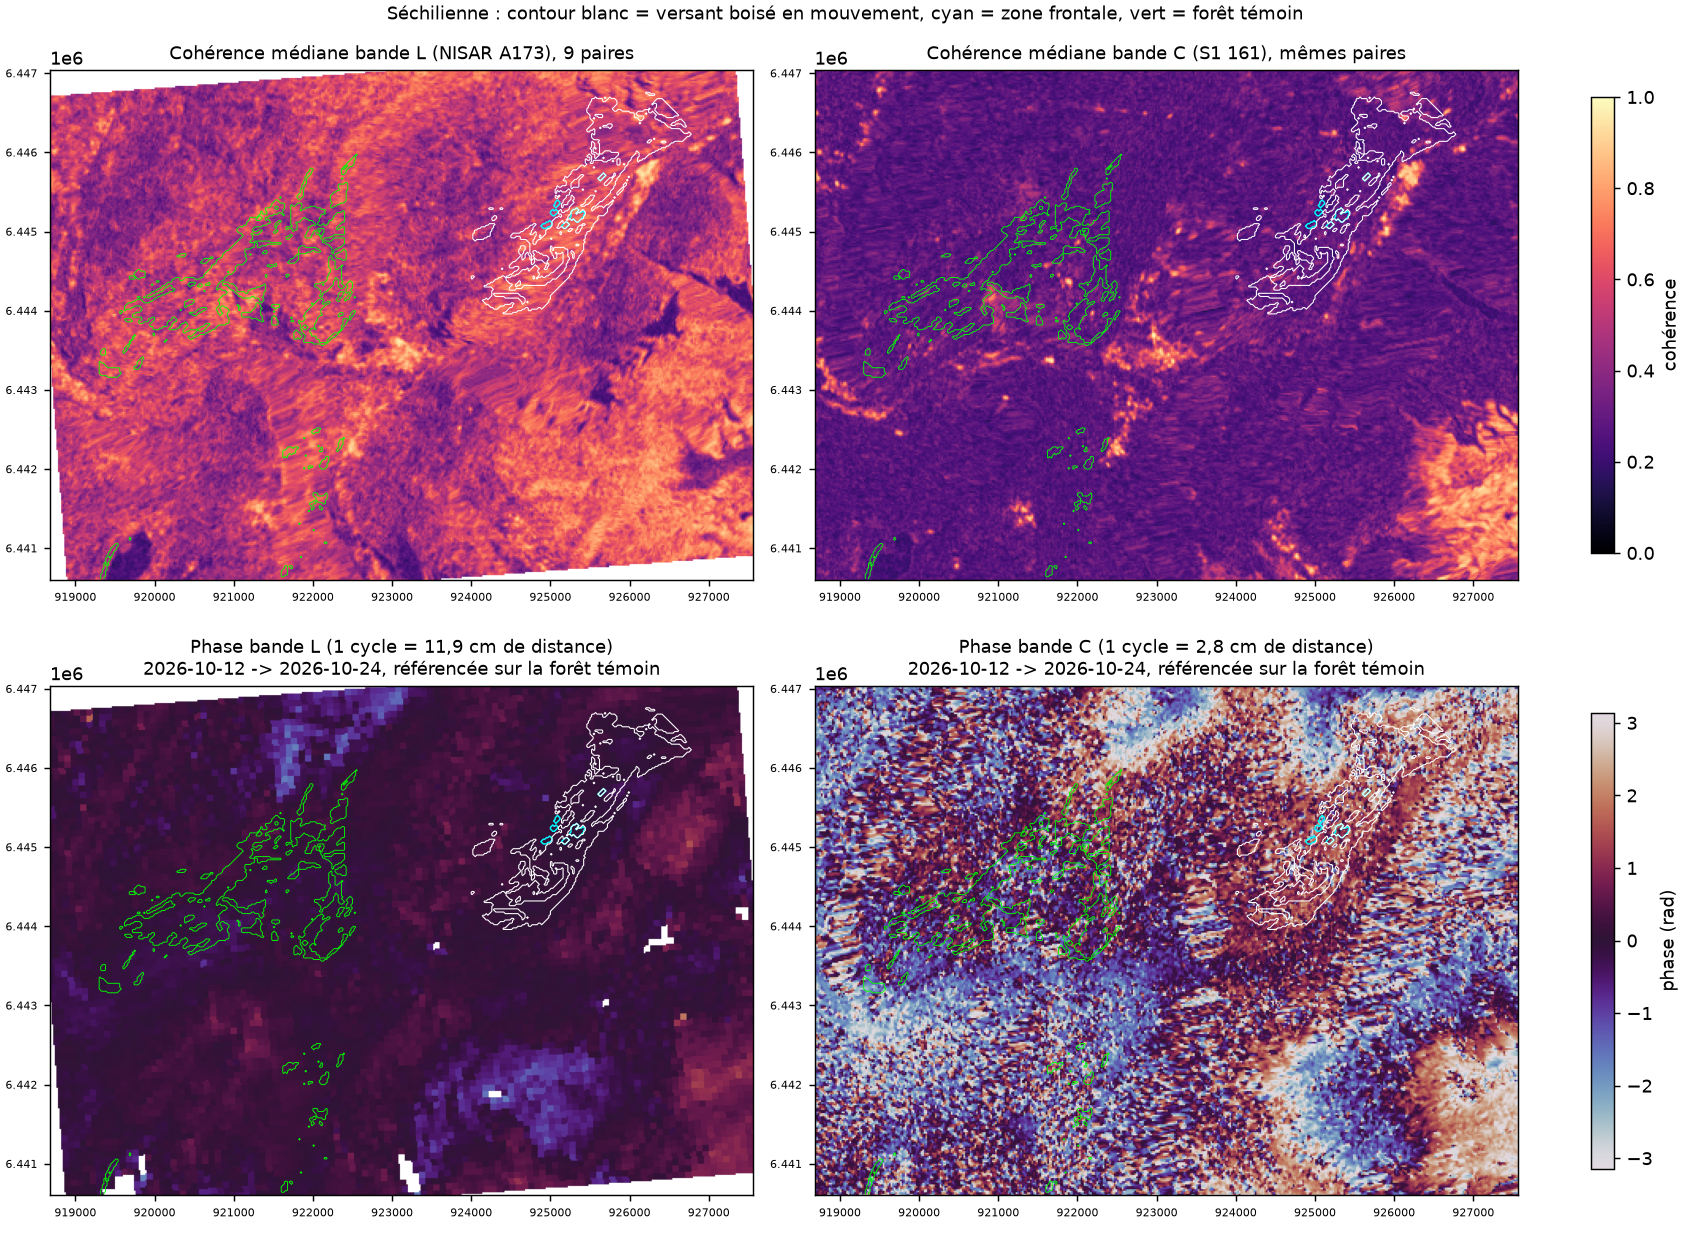
\includegraphics[width=0.80\linewidth, height=0.74\textheight, keepaspectratio]{g4_maps_A173.png}

	\scriptsize Phase \Lb{L} lisse et cohérente sous la forêt ; phase \Cb{C} aléatoire hors bâti et éboulis.
\end{frame}

\begin{frame}{\phantom{x}}
	\frametitle{Résultats (2/3) : la phase sous la forêt}
	\vspace{-4pt}\scriptsize
	\centering
	\begin{tabular}{lcccc}
		\toprule
		Médiane (min--max) & \Lb{L A173} & \Cb{C A161} & \Lb{L D138} & \Cb{C D139}\\
		\midrule
		Cohérence, versant & \textbf{0,58} (0,38--0,81) & 0,28 & 0,32 & 0,29\\
		Cohérence, témoin & \textbf{0,60} & 0,27 & 0,43 & 0,28\\
		Consistance, versant & \textbf{0,92} (0,79--0,99) & 0,11 (0,00--0,53) & \textbf{0,88} & 0,09\\
		Consistance, frontale & \textbf{0,97} & 0,27 & masquée & 0,28\\
		\bottomrule
	\end{tabular}

	\vspace{10pt}
	\keynum{Lband}{0,92}{consistance de phase \Lb{L}\\versant boisé (montante)}\hfill
	\keynum{Cband}{0,11}{consistance de phase \Cb{C}\\même versant, mêmes dates}\hfill
	\keynum{myblue}{0,27}{cohérence \Cb{C} en forêt\\= plancher de biais}

	\vspace{8pt}
	\raggedright
	\Cb{C} décorrélée par le feuillage à 12~jours \parencite{zebker1992decorrelation} ;
	la descendante est défavorable (versant opposé à la visée).
\end{frame}

\begin{frame}{\phantom{x}}
	\frametitle{Résultats (3/3) : déplacement en bande L}
	\vspace{-6pt}
	\centering
	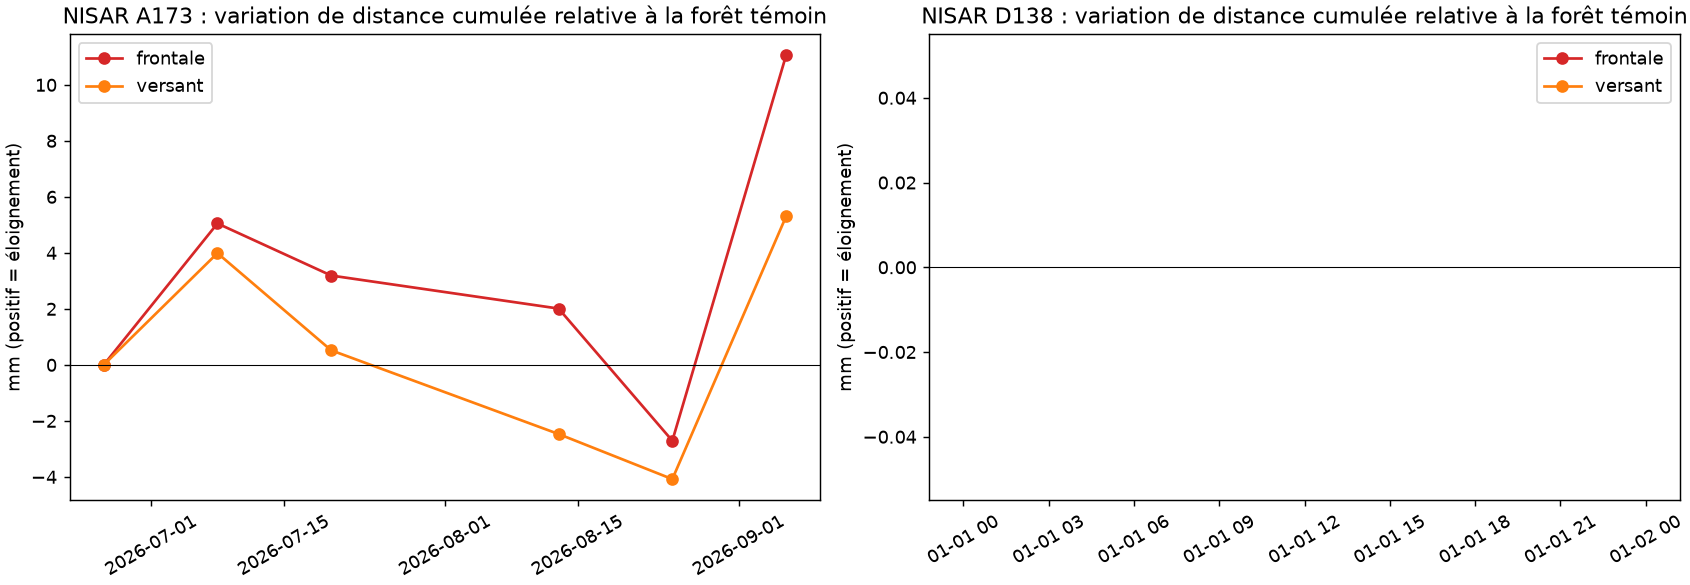
\includegraphics[width=0.92\linewidth, height=0.52\textheight, keepaspectratio]{g4_cumul_L.png}

	\scriptsize\raggedright
	\begin{itemize}
		\setlength{\itemsep}{0pt}
		\item Versant : de $-4$ à +5~mm cumulés sur 4 mois, \textbf{sans tendance} ; dispersion du témoin 3--10~mm par paire
		\item 1--5~cm/an représentent < 1~cm en 4 mois : \textbf{sous le bruit} d'une paire isolée
		\item Compatible avec un glissement aujourd'hui lent, sans rien démontrer sur sa vitesse
	\end{itemize}
\end{frame}

% ================================================================
\section{Conclusion}
% ================================================================

\begin{frame}{\phantom{x}}
	\frametitle{Conclusion, limites et perspectives}
	\vspace{-6pt}\scriptsize
	\begin{exampleblock}{Conclusion}
		\scriptsize
		Sous la forêt, \Lb{NISAR} garde une phase consistante (0,8--1) ; \Cb{Sentinel-1} non.
		La condition nécessaire à l'interférométrie de déplacement est remplie en \Lb{L} seulement :
		argument pour NISAR puis \textbf{ROSE-L} \parencite{esa2020rosel}.
	\end{exampleblock}
	\begin{columns}[T]
		\column{0.49\textwidth}
		\begin{alertblock}{Limites}
			\scriptsize
			\begin{itemize}
				\setlength{\itemsep}{0pt}
				\item Un seul site, mouvement lent, 4 mois
				\item Pas de données au sol 2026
				\item Zones issues de la littérature et de l'imagerie
				\item Descendante peu exploitable ; \Cb{C} en VV seulement
			\end{itemize}
		\end{alertblock}
		\column{0.49\textwidth}
		\begin{block}{Perspectives}
			\scriptsize
			\begin{itemize}
				\setlength{\itemsep}{0pt}
				\item Série NISAR $\geq$ 1 an, inversion SBAS (écosystème ISCE3)
				\item Comparaison aux mesures géodésiques du site
				\item Chaîne indépendante du capteur, prête pour ROSE-L
			\end{itemize}
		\end{block}
	\end{columns}
\end{frame}

\begin{frame}[allowframebreaks]{Références}
	\scriptsize
	\printbibliography[heading=none]
\end{frame}

\end{document}
